\section{Extended Ablation Studies}
\label{sec:ablations}

\subsection*{Feature Group Ablation}

\begin{table}[htb]
\centering
\small
\setlength{\tabcolsep}{4pt}
\renewcommand{\arraystretch}{0.95}
\caption{\textbf{Feature group ablation (Pixtral-12B, VQA-v2).}
\texttt{tfidf+struct} is the full \textsc{VOILA} feature set (5,017 dims).}
\label{tab:feature_ablation_appendix}
\begin{tabular}{lrcc}
\toprule
\textbf{Feature set} & \textbf{Dims} & \textbf{Acc\%} & \textbf{Cost} \\
\midrule
TF-IDF only          & 5{,}000 & 66.1 & 45.2 \\
Question-type flags only & 5   & 69.1 & 50.5 \\
Lexical stats only   & 12      & 65.4 & 40.3 \\
TF-IDF + struct (\textsc{VOILA}) & 5{,}017 & \textbf{64.1} & \textbf{38.7} \\
\bottomrule
\end{tabular}
\end{table}

\subsection*{TF-IDF Feature Importances}

\begin{figure}[htb]
\centering
\subfloat[Caption sufficiency]{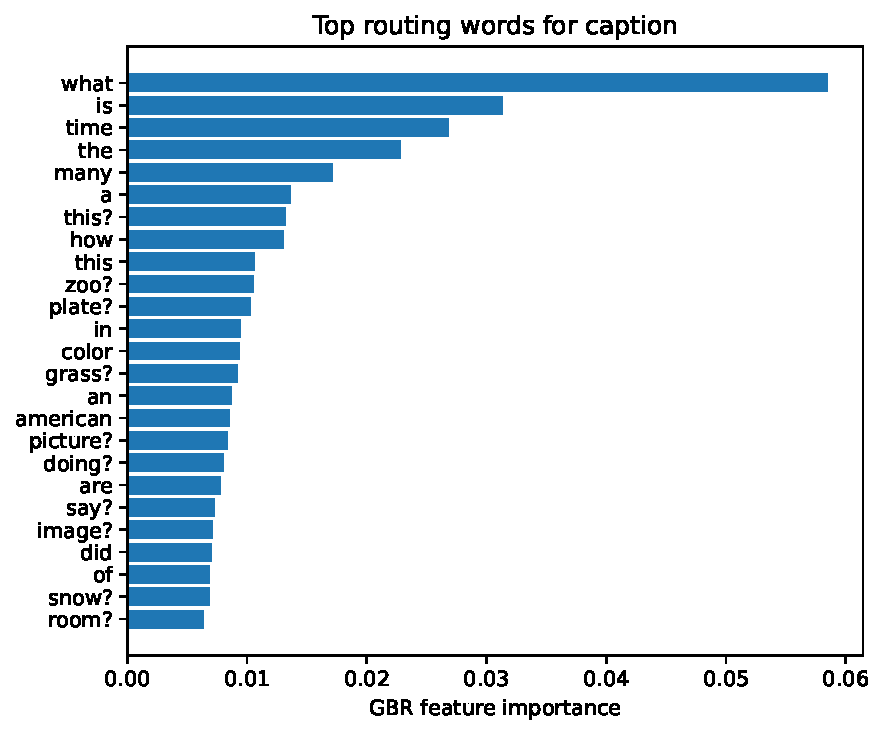
\includegraphics[width=0.49\linewidth]{plots/routing_words_caption.pdf}}
\hfill
\subfloat[Full-resolution need]{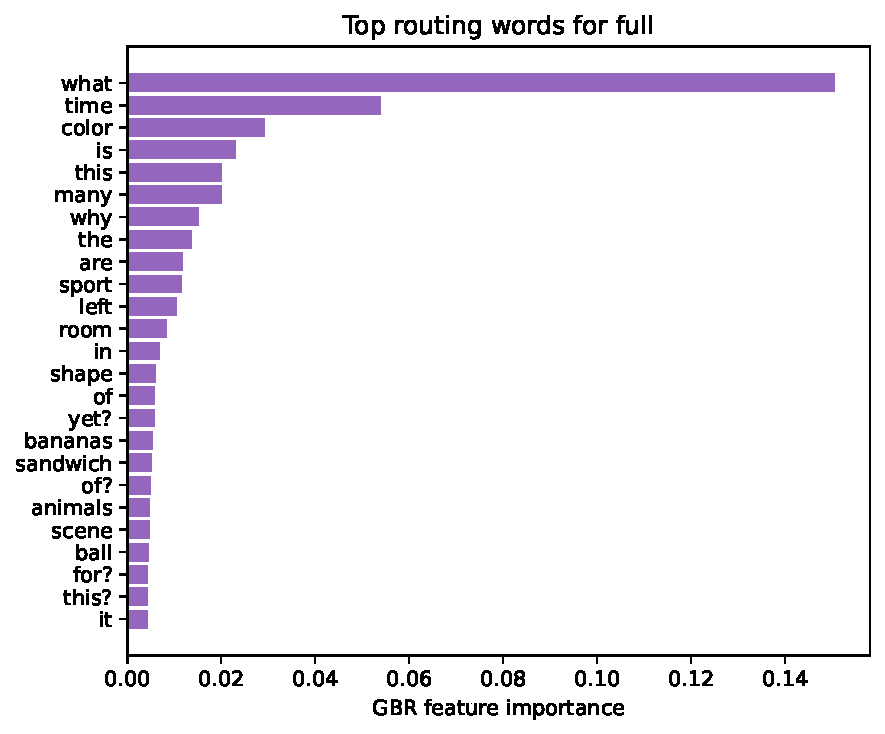
\includegraphics[width=0.49\linewidth]{plots/routing_words_full.pdf}}
\caption{\textbf{Top TF-IDF feature importances} learned by the GBR routing model (VQA-v2, Pixtral-12B). Words predictive of caption-level sufficiency (left) skew toward semantically coarse queries (\emph{is}, \emph{there}); those predicting full-resolution need (right) include visually specific terms (\emph{color}, \emph{many}, \emph{sport}).}
\label{fig:routing_words}
\end{figure}

\subsection*{Iso-Accuracy Contours: Fidelity vs.\ Model Scale}

\begin{figure}[htb]
\centering
\subfloat[VQA-v2]{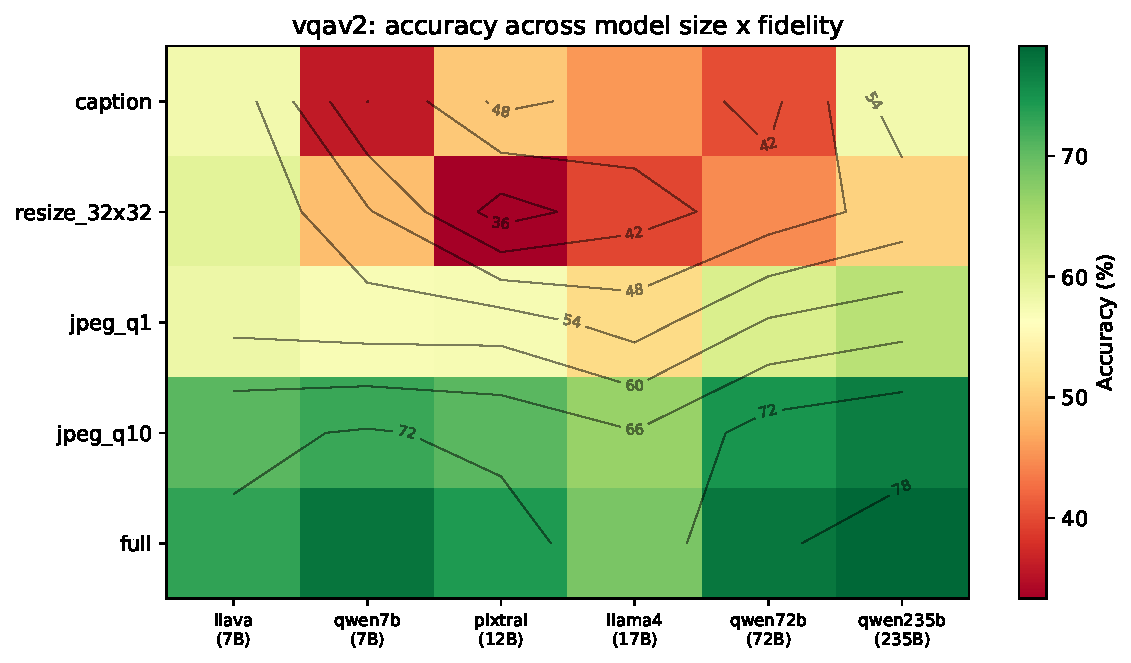
\includegraphics[width=0.49\linewidth]{plots/iso_accuracy_contour_vqav2.pdf}}
\hfill
\subfloat[GQA]{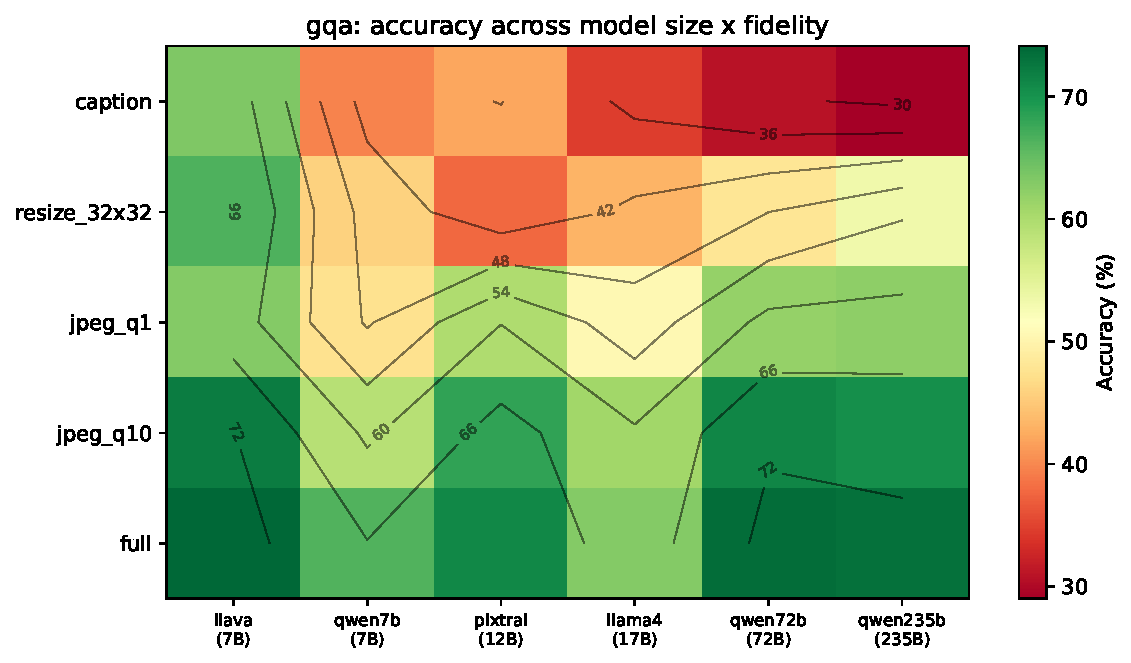
\includegraphics[width=0.49\linewidth]{plots/iso_accuracy_contour_gqa.pdf}}
\caption{\textbf{Iso-accuracy contours} showing VQA accuracy as a joint function of model scale and input fidelity. Contour lines connect (model, fidelity) pairs achieving equal accuracy. Fidelity improvements provide gains comparable to large model-scale jumps: a 7B model at JPEG Q10 often matches a 235B model at caption fidelity (Observation~3). The contours quantify why fidelity and model capacity are complementary, not substitutable, optimization dimensions.}
\label{fig:iso_accuracy_contour}
\end{figure}

\subsection*{Reliability Diagrams: Calibration Quality Across Settings}

\begin{figure}[htb]
\centering
\subfloat[VQA-v2 / Pixtral-12B]{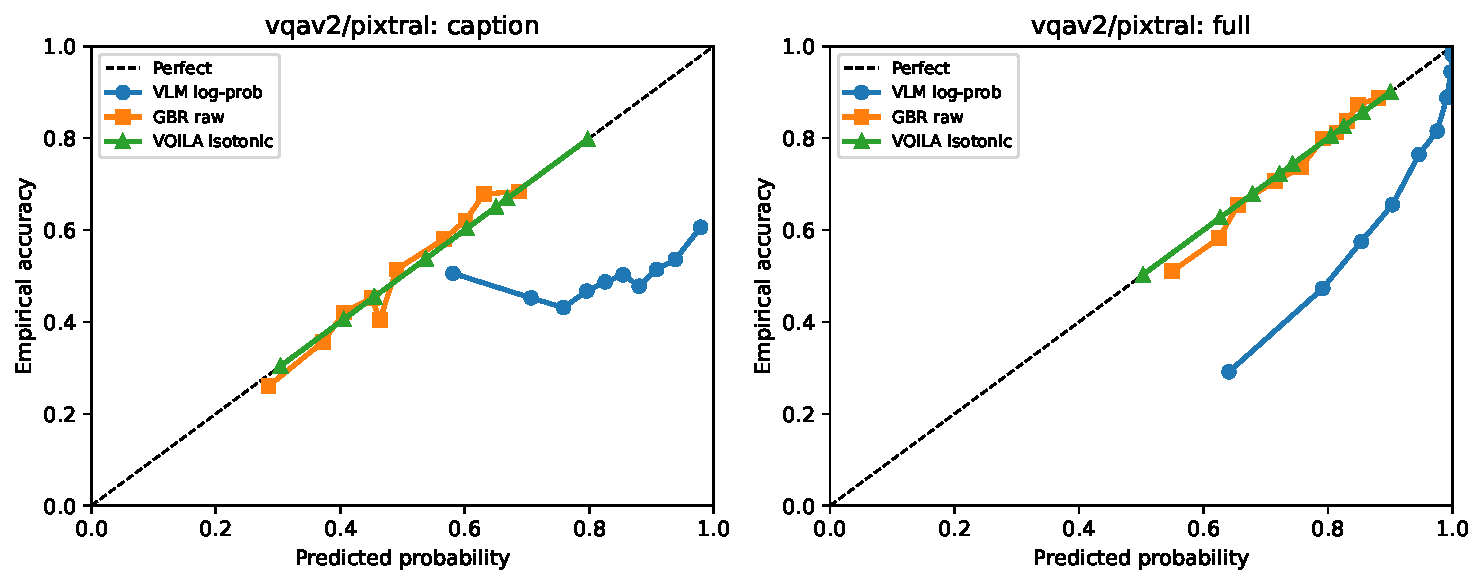
\includegraphics[width=0.49\linewidth]{plots/reliability_vqav2_pixtral.pdf}}
\hfill
\subfloat[GQA / Qwen2.5-VL-7B]{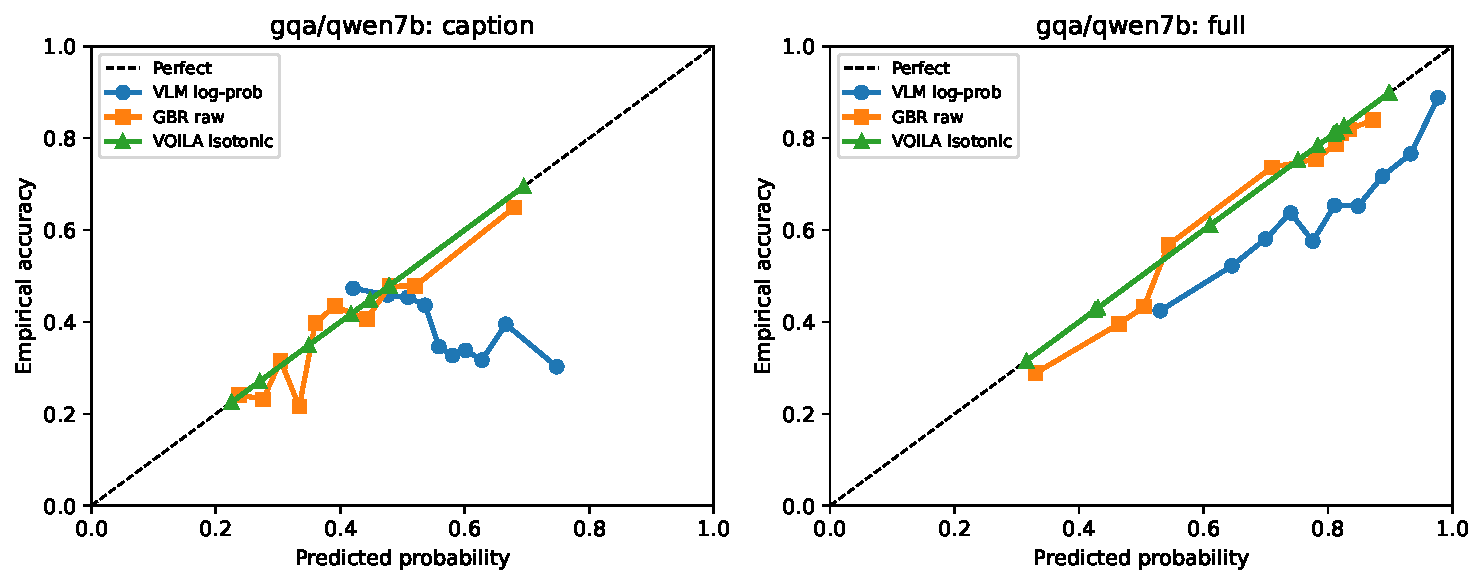
\includegraphics[width=0.49\linewidth]{plots/reliability_gqa_qwen7b.pdf}}
\caption{\textbf{Reliability diagrams} comparing VLM log-probability confidence, raw GBR scores, and isotonic-calibrated VOILA probabilities against the perfect-calibration diagonal (dashed). Isotonic calibration closely tracks the diagonal across both model--dataset pairs; ECE reduces from 0.025 to 0.012 (VQA-v2/Pixtral) and from 0.042 to 0.020 (GQA/Qwen7B).}
\label{fig:reliability}
\end{figure}

\subsection*{Score Separation: Calibrated vs.\ Uncalibrated Predictions}

\begin{figure}[htb]
\centering
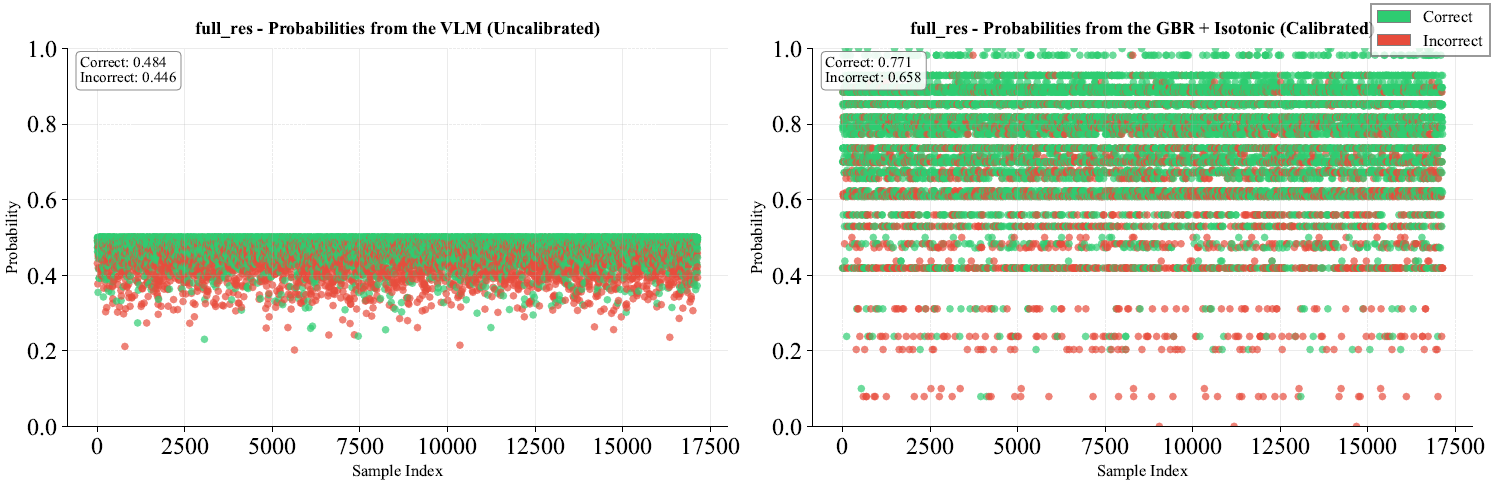
\includegraphics[width=\linewidth]{plots/calibration_uncalibration_img.png}
\caption{\textbf{Score separation before and after isotonic calibration} (VQA-v2, Pixtral-12B, caption fidelity). Each point is a query, colored by outcome (correct/incorrect). Raw GBR scores overlap substantially between correct and incorrect predictions, making threshold-based escalation unreliable. After isotonic calibration, correct predictions cluster toward higher probabilities and incorrect predictions toward lower values, enabling reliable expected-value computations in the VOI criterion.}
\label{fig:calibration_scatter}
\end{figure}

\subsection*{ROC Curves for Escalation Decisions}

\begin{figure}[htb]
\centering
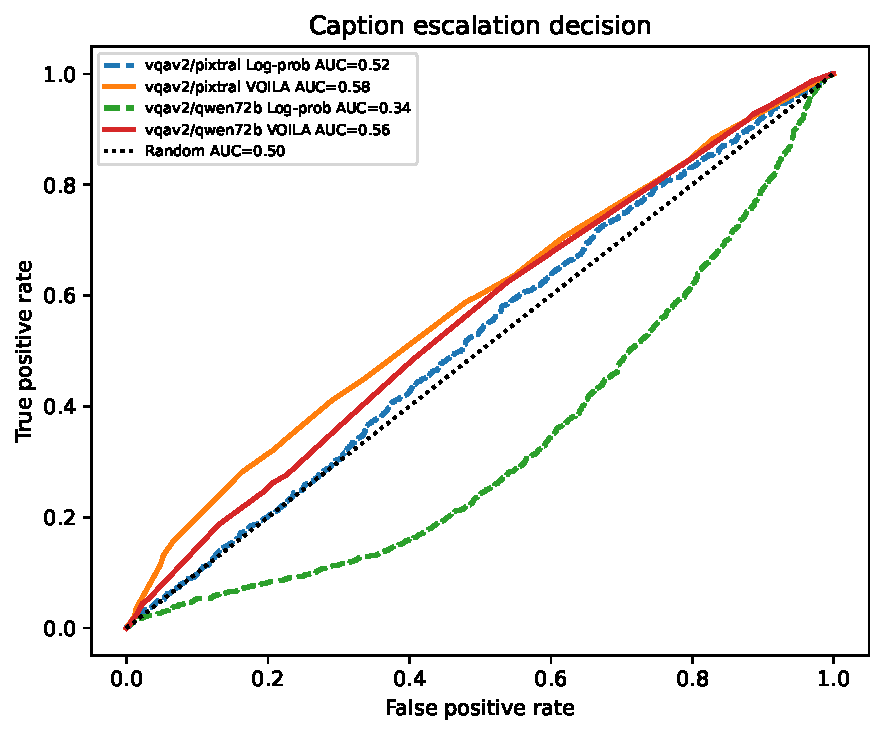
\includegraphics[width=0.92\linewidth]{plots/roc_escalation_decision.pdf}
\caption{\textbf{ROC curves for caption-to-full escalation decisions} (VQA-v2). A positive example is a query where caption fidelity fails but full resolution succeeds. \textsc{VOILA}'s question-conditioned score (AUC\,=\,0.581) outperforms log-probability thresholding (AUC\,=\,0.522) for Pixtral-12B. For Qwen2-VL-72B, the log-probability AUC falls to 0.338---below random (dashed)---confirming that VLM confidence is actively anti-correlated with the need to escalate for this model.}
\label{fig:roc_escalation}
\end{figure}

\begin{table*}[p]
\centering
\tiny
\caption{
\textbf{Extended Calibration Ablation Across All Models (VQA-v2 and GQA).}
Each entry reports \textbf{Acc (\%) / Cost}.
We evaluate three calibration methods (None, Isotonic, Temperature Scaling) and two alternative decision rules (Accuracy-only, Fixed-threshold) across six VLMs.
\emph{Iso} (isotonic, \textsc{VOILA} default) is bolded; it consistently achieves the strongest cost--accuracy Pareto position.
Fixed-resolution cost is 100; all other costs are normalized relative to this.
}
\label{tab:extended_ablation_all}\label{tab:ablation_calibration}
\resizebox{\linewidth}{!}{
\begin{tabular}{llccccc}
\toprule
\multirow{2}{*}{\textbf{Model}} & \multirow{2}{*}{\textbf{Method}}
& \multicolumn{3}{c}{\textbf{Calibration Variants (VOI Routing)}}
& \multicolumn{2}{c}{\textbf{Alternative Decision Rules (Isotonic)}} \\
\cmidrule(lr){3-5}\cmidrule(lr){6-7}
& & \textbf{None} & \textbf{Isotonic} & \textbf{Temp. Scaling}
& \textbf{Acc-only} & \textbf{Fixed-Thr.} \\
\midrule
\multicolumn{7}{c}{\textit{\textbf{VQA-v2}}} \\
\midrule
Pixtral-12B
& Acc / Cost
& 67.4 / 47.6
& \textbf{64.1 / 38.7}
& 66.5 / 45.3
& 74.2 / 100.0
& 59.7 / 32.2 \\

Llama-4-Maverick
& Acc / Cost
& 60.5 / 38.5
& \textbf{59.7 / 37.1}
& 60.7 / 39.6
& 68.4 / 100.0
& 56.6 / 33.9 \\

Qwen2-VL-72B
& Acc / Cost
& 67.3 / 43.2
& \textbf{64.4 / 37.3}
& 65.8 / 40.7
& 77.6 / 100.0
& 57.8 / 31.0 \\

LLaVA-1.5-7B
& Acc / Cost
& 67.9 / 34.5
& \textbf{66.5 / 26.2}
& 67.8 / 32.7
& 73.1 / 100.0
& 62.5 / 18.0 \\

Qwen2.5-VL-7B
& Acc / Cost
& 63.4 / 34.3
& \textbf{63.1 / 34.1}
& 64.3 / 36.7
& 77.8 / 100.0
& 61.4 / 33.5 \\

Qwen3-VL-235B
& Acc / Cost
& 71.1 / 33.6
& \textbf{71.5 / 37.4}
& 71.3 / 34.6
& 79.1 / 100.0
& 62.9 / 17.5 \\

\midrule
\multicolumn{7}{c}{\textit{\textbf{GQA}}} \\
\midrule
Pixtral-12B
& Acc / Cost
& 61.2 / 32.6
& \textbf{60.4 / 31.1}
& 61.1 / 31.4
& 71.1 / 100.0
& 59.1 / 34.5 \\

Llama-4-Maverick
& Acc / Cost
& 52.3 / 26.2
& \textbf{53.4 / 29.5}
& 53.5 / 29.4
& 62.9 / 100.0
& 53.7 / 40.0 \\

Qwen2-VL-72B
& Acc / Cost
& 60.1 / 30.8
& \textbf{60.0 / 28.9}
& 60.3 / 30.5
& 73.5 / 100.0
& 58.3 / 30.7 \\

LLaVA-1.5-7B
& Acc / Cost
& 70.0 / 29.3
& \textbf{69.5 / 25.9}
& 70.0 / 30.4
& 74.1 / 100.0
& 65.0 / 12.1 \\

Qwen2.5-VL-7B
& Acc / Cost
& 57.2 / 33.5
& \textbf{55.0 / 27.8}
& 56.7 / 32.8
& 66.2 / 100.0
& 53.2 / 47.0 \\

Qwen3-VL-235B
& Acc / Cost
& 59.9 / 26.8
& \textbf{59.0 / 24.3}
& 59.4 / 24.1
& 73.2 / 100.0
& 59.9 / 32.3 \\

\bottomrule
\end{tabular}
}
\end{table*}

\begin{table}[p]
\centering
\small
\caption{
\textbf{Predictor Robustness Under Fixed Isotonic Calibration (Pixtral-12B).}
Each entry reports \textbf{Acc (\%) / Cost}.
Performance is broadly similar across predictor architectures once calibration is applied, demonstrating that \textsc{VOILA}'s gains stem from calibration and VOI routing rather than predictor choice.
GBR (\textsc{VOILA} default) is bolded.
}
\label{tab:predictor_robustness_extended}
\label{tab:predictor_robustness_pixtral}
\setlength{\tabcolsep}{5pt}
\begin{tabular}{lcccc}
\toprule
\textbf{Dataset} & \textbf{GBR} & \textbf{LogReg} & \textbf{Ridge} & \textbf{MLP} \\
\midrule
VQA-v2 & \textbf{64.1 / 38.8} & 65.0 / 43.4 & 63.9 / 40.0 & 63.4 / 38.4 \\
GQA    & \textbf{60.5 / 31.1} & 60.2 / 30.6 & 59.6 / 29.9 & 60.3 / 31.6 \\
\bottomrule
\end{tabular}
\end{table}


This section provides a comprehensive analysis of \textsc{VOILA}'s design choices, expanding on the ablation results summarized in the main paper.
We evaluate calibration methods and decision rules across six VLMs and two datasets (VQA-v2 and GQA), and assess predictor robustness for Pixtral-12B.

\subsection{Experimental Design}
\label{sec:ablation_design}

We evaluate three dimensions of design choices:

\textbf{Calibration methods.} We compare three approaches to converting raw predictor scores into probabilities suitable for utility estimation:
\begin{itemize}[leftmargin=*,nosep]
\item \textit{None}: Raw GBR scores used directly without post-hoc calibration.
\item \textit{Isotonic}: Isotonic regression applied to raw scores (\textsc{VOILA} default), enforcing monotonicity while remaining non-parametric.
\item \textit{Temperature scaling}: A standard post-hoc calibration method from classification literature~\cite{guo2017calibrationmodernneuralnetworks}, included as a negative control.
\end{itemize}

\textbf{Decision rules.} Given calibrated predictors, we compare VOI routing against two alternative strategies:
\begin{itemize}[leftmargin=*,nosep]
\item \textit{Accuracy-only}: Always select the fidelity with highest predicted correctness probability, ignoring acquisition cost. Represents an unconstrained accuracy-maximizing baseline.
\item \textit{Fixed-threshold}: Escalate to higher fidelity only when predicted probability falls below a fixed cutoff tuned on held-out VQA-v2 data.
\end{itemize}

\textbf{Predictor architectures.} We evaluate four question-conditioned regressors under fixed isotonic calibration for Pixtral-12B: Gradient Boosting (GBR, \textsc{VOILA} default), Logistic Regression, Ridge Regression, and MLP. All use identical question features.

\subsection{Comprehensive Results}
\label{sec:ablation_results}

Table~\ref{tab:extended_ablation_all} reports accuracy and cost for each ablation across 12 model--dataset combinations.

\paragraph{Isotonic calibration consistently improves the cost--accuracy tradeoff.}
Comparing columns 1--2 in Table~\ref{tab:extended_ablation_all}, isotonic calibration achieves lower cost than uncalibrated routing while maintaining comparable accuracy.
For example, on VQA-v2 with LLaVA-1.5-7B, uncalibrated routing achieves 67.9\% at cost 34.5, whereas isotonic calibration achieves 66.5\% at cost 26.2 --- a 24\% cost reduction with only 1.4 point accuracy sacrifice.
On GQA with Pixtral-12B, isotonic routing achieves 60.4\% at cost 31.1 versus uncalibrated 61.2\% at cost 32.6.
The advantage is most pronounced when predictions are overconfident at low fidelity: calibration corrects this, reducing unnecessary escalation.

\paragraph{Calibration improves routing efficiency, not task accuracy.}
Calibration does not alter which visual information is processed or how the VLM reasons; it improves \emph{routing decisions} by producing reliable probability estimates.
Isotonic regression's monotonicity constraint ensures that utility differences $\hat{p}_{k+1}(q) - \hat{p}_k(q)$ reliably indicate when escalation is beneficial, a property that general-purpose calibrators like temperature scaling do not enforce.

\paragraph{Temperature scaling is not appropriate for cost-sensitive sequential decisions.}
Temperature scaling (column 3) often increases cost relative to isotonic calibration without accuracy gains.
On VQA-v2 with Pixtral, temperature scaling achieves 66.5\% at cost 45.3 versus isotonic's 64.1\% at cost 38.7 --- 17\% higher cost.
The instability reflects temperature scaling's optimization of global calibration metrics (log-loss) that do not align with cross-fidelity utility ordering.

\subsection{Why VOI Routing Dominates Heuristic Baselines}
\label{sec:voi_dominance}

\paragraph{Accuracy-only selection: the cost of ignoring resources.}
The accuracy-only baseline (column 4) always retrieves at cost 100 (full resolution by construction), representing 60--170\% cost inflation over \textsc{VOILA} depending on the setting.
The accuracy gain is marginal: for Qwen3-VL-235B on VQA-v2, accuracy-only achieves 79.1\% versus \textsc{VOILA}'s 71.5\% --- an 7.6 point gap at 170\% cost inflation.
For LLaVA-1.5-7B on GQA, the gap is only 4.6 points (74.1\% vs.\ 69.5\%) at 286\% cost inflation, confirming that most queries do not require maximum-fidelity inputs.

\paragraph{Fixed-threshold heuristics: brittleness without adaptivity.}
The fixed-threshold baseline (column 5) shows inconsistent behavior across settings.
On GQA with LLaVA-1.5-7B, it achieves 65.0\% at cost 12.1 --- lower cost than \textsc{VOILA}'s 69.5\% at 25.9 but with 4.5 point accuracy loss, suggesting over-aggressive escalation avoidance.
On GQA with Qwen2.5-VL-7B, it achieves 53.2\% at cost 47.0 --- higher cost than \textsc{VOILA}'s 55.0\% at 27.8 with 1.8 point accuracy loss, showing under-escalation on visually demanding queries.
This dataset- and model-dependent behavior requires per-setting retuning, whereas \textsc{VOILA}'s VOI criterion adapts automatically.

\subsection{Robustness to Predictor Architecture}
\label{sec:predictor_robustness}

Table~\ref{tab:predictor_robustness_extended} evaluates four predictors for Pixtral-12B under isotonic calibration.
On VQA-v2, GBR achieves 64.1\% at cost 38.8 while LogReg achieves 65.0\% at cost 43.4, Ridge achieves 63.9\% at cost 40.0, and MLP achieves 63.4\% at cost 38.4.
The accuracy spread (1.6 points) and cost spread (5.0 units) are small relative to the gains from calibration itself.
On GQA, the spread is even smaller: 60.2--60.5\% accuracy and 29.9--31.6 cost.
This robustness validates that \textsc{VOILA}'s performance is driven by calibration quality and VOI routing, not predictor expressivity.
System designers can choose predictors based on deployment constraints (memory, latency, retraining frequency) without sacrificing core benefits.

\subsection{Key Takeaways and Design Implications}
\label{sec:takeaways}

Our extended ablation studies establish four findings:

\textbf{(1) Calibration is essential, but method choice matters.}
Isotonic regression is well-suited for cost-sensitive sequential decisions because it enforces cross-fidelity monotonicity.
General-purpose methods like temperature scaling optimize global metrics that do not align with routing quality.

\textbf{(2) VOI routing dominates heuristics across the cost--accuracy frontier.}
Accuracy-only selection over-retrieves; fixed thresholds under- or over-retrieve unpredictably.
\textsc{VOILA} achieves Pareto optimality by reasoning about marginal utility via calibrated probabilities, without per-dataset retuning.

\textbf{(3) \textsc{VOILA} is robust to implementation choices.}
The same pipeline yields consistent gains across six VLMs (7B--235B), two datasets, and four predictor architectures.

\textbf{(4) The framework is complementary to model routing.}
\textsc{VOILA} optimizes \emph{what to retrieve before model execution}; model routing optimizes \emph{which model to apply after retrieval}.
These axes are orthogonal and can be combined for end-to-end efficiency in multimodal systems.

\subsection*{Log-prob Cascade Degeneracy}

\begin{table}[htb]
\centering
\small
\setlength{\tabcolsep}{3pt}
\caption{\textbf{Log-prob Cascade degeneracy} (representative cases). Near-zero escalation rates indicate the cascade never leaves caption fidelity (underconfidence failure); near-100\% rates indicate it always escalates to full resolution (overconfidence failure). Averaged across all 24 model--dataset pairs, the cascade escalates in 50\% of queries at cost 39.7, vs.\ \textsc{VOILA}'s cost of 27.3.}
\label{tab:cascade_degeneracy}
\begin{tabular}{llcc}
\toprule
\textbf{Model} & \textbf{Dataset} & \textbf{Escalation rate} & \textbf{Avg.\ cost} \\
\midrule
\multicolumn{4}{l}{\textit{Degenerate: never escalates}} \\
Qwen2-VL-72B  & TextVQA & 0.00\% & 7.6 \\
Qwen2-VL-72B  & GQA     & 0.03\% & 7.6 \\
Qwen2-VL-72B  & VQA-v2  & 0.18\% & 7.7 \\
LLaMA-4-Mav.  & GQA     & 0.28\% & 7.8 \\
\midrule
\multicolumn{4}{l}{\textit{Degenerate: always escalates}} \\
Qwen3-VL-235B & GQA     & 99.96\% & 83.8 \\
Qwen2.5-VL-7B & GQA     & 99.78\% & 74.8 \\
\midrule
\textit{Overall avg.} & all & 50.0\% & 39.7 \\
\bottomrule
\end{tabular}
\end{table}
